%% chapter one draft.
\chapter{Big Data and Hadoop}\label{chap:1}
In this chapter, we will cover:
\begin{itemize}
  \item Defining a Big Data problem
  \item Building a Hadoop based Big Data platform
  \item Choosing from Hadoop alternatives
\end{itemize}

\section{Introduction}\label{chap1:intro}
Today, many organizations are facing the Big Data problem. Managing and processing Big Data can incur a lot of challenges for traditional data processing platforms such as relational database systems. Hadoop was designed to be a distributed and scalable system for dealing with Big Data problems.

The design, implementation and deployment of a Big Data platform require a clear definition of the Big Data problem by system architects and administrators etc. A Hadoop based Big Data platform uses Hadoop as the data storage and processing engine. It deals with the problem by transforming the Big Data input into expected output. On the one hand, the Big Data problem determines how the Big Data platform should be designed, for example, which modules or subsystems should be integrated into the platform and so on. On the other hand, the architectural design of the platform can determine complexity and efficiency of the platform.

Different Big Data problems have different properties. A Hadoop based Big Data platform is capable of dealing with most of the Big Data problems, while not good fit for others. Because of these and many other reasons, we need to choose from Hadoop alternatives.

\section{Defining a Big Data Problem}\label{chap1:problem}
Generally, the definition of Big Data\index{Big Data|textbf} is that data with sizes go beyond the ability of commonly-used software tools to collect, manage, and process within a tolerable elapsed time. More formally, the definition of Big Data should go beyond the size of the data to include other properties. In this recipe, we will outline the properties that define Big Data in a formal way.

\subsection*{Getting ready}
Formally, data has the following three important properties: volume, velocity and variety. In this book, we treat the value property of Big Data as the fourth important property. And the value property also explains the reason why Big Data problem exists.

\subsection*{How to do it}
Defining a Big Data problem involves the following steps:
\begin{enumerate}
  \item Estimate the volume of data. The volume should not only include the current data volume for example in gigabytes or terabytes, but also should include the expected volume in the future. There are two types of data in real world: static and non-static data. The volume of static data, for example national census data and human genomic data, will not change over time. While for non-static data, such as streaming log data and social network streaming data, the volume are increasing over time.
  \item Estimate the velocity of data. The velocity estimate should include how much data can be generated within a certain amount of time, for example during a day. For static data, the velocity is zero. The velocity property of Big Data defines the speed that data can be generated. This property will not only affect the volume of data but also determines how fast a data processing system should handle the data.
  \item Identify the data variety. In other words, the data variety means the different sources of data, such as web click data, social network data and data in relational databases etc. Variety means that data differs syntactically or semantically. The difference requires specifically designed modules for each data variety to be integrated into the Big Data platform. For example, a web crawler is needed for getting data from the web and a data translation module is needed to transfer data from relational databases to a non-relational Big Data platform.
  \item Define the expected value of data. The value property of Big Data defines what we can potentially derive from and how we can use Big Data. For example, frequent item sets can be mined from online click-through data for better marketing and more efficient deployment of advertisements.
\end{enumerate}

\subsection*{How it works}
A Big Data platform can be described with the \href{http://en.wikipedia.org/wiki/IPO_Model}{IPO} model, which includes three components: input, process and output. For a Big Data problem, the volume, velocity and variety properties together define the input of the system and the value property defines the output.
\subsection*{See also}
\begin{itemize}
  \item Building a Hadoop based Big Data platform
\end{itemize}
\section{Building a Hadoop based Big Data platform}
Hadoop was first developed as a Big Data processing system in 2006 at Yahoo! The idea is based on Google's MapReduce\index{MapReduce}, which was first published by Google based on their proprietary MapReduce implementation. In the past few years, Hadoop has become a widely used platform and runtime environment for the deployment of Big Data applications. In this recipe, we will outline steps to build a Hadoop based Big Data platform.
\subsection*{Getting ready}
Hadoop was designed to be parallel and resilient. It redefines the way that data is managed and processed by leveraging the power of computing resources composed of commodity hardware. And it can automatically recover from failures.
\subsection*{How to do it}
Use the following steps to build a Hadoop based Big Data platform:
\begin{enumerate}
  \item Design, implement and deploy data collection or aggregation subsystems. The subsystems should transfer data from different data sources to Hadoop compatible data storage systems such as HDFS and HBase. The subsystems need to be designed based on the input properties of a Big Data problem including volume, velocity and variety.
  \item Design, implement and deploy Hadoop Big Data processing platform. The platform should consume the Big Data located on HDFS or HBase and produce the expected and valuable output.
  \item Design, implement and deploy result delivery subsystems. The delivery subsystems should transform the analytical results from a Hadoop compatible format to a proper format for end users. For example, we can design web applications to visualize the analytical results using charts, graphs or other types of dynamic web applications.
\end{enumerate}
\subsection*{How it works}
The architecture of a Hadoop based Big Data system can be described with the following figure:

\begin{figure}[h]
  \centering
  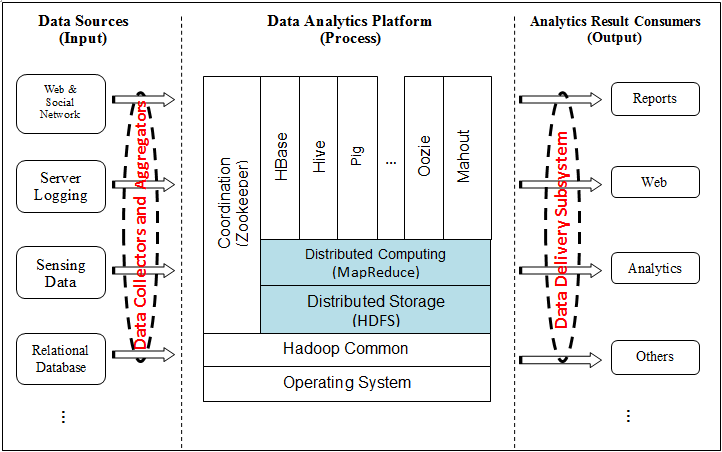
\includegraphics[width=\textwidth]{figs/5163os_01_01.png}
  \caption{Architecture of Hadoop based big data system}\label{fig:hadoop.architecture}
\end{figure} 

%%\verb|Insert image 5163os_01_01.png|

Although Hadoop borrows its idea from Google's MapReduce, it is more than MapReduce. A typical Hadoop based Big Data platform includes the Hadoop Distributed File System (HDFS\index{HDFS}), the parallel computing framework (MapReduce\index{MapReduce}) , common utilities, a column oriented data storage table (HBase\index{HBase}), high level data management systems (Pig\index{Pig} and Hive\index{Hive}), a Big Data analytics library (Mahout\index{Mahout}), a distributed coordination system (ZooKeeper\index{ZooKeeper}), a workflow management module (Oozie\index{Oozie}), data transfer modules such as Sqoop\index{Sqoop}, data aggregation modules such as Flume\index{Flume} and data serialization modules such as Avro\index{Avro}.

HDFS is the default filesystem of Hadoop. It was designed as a distributed filesystem that provides high-throughput access to application data. Data on HDFS is stored as data blocks. The data blocks are replicated on several computing nodes and their checksums are computed. In case of checksum error or system failure, erroneous or lost data blocks can be recovered from backup blocks located on other nodes.

MapReduce\index{MapReduce} provides a programming model that transforms complex computations into computations over a set of key-value pairs. It coordinates the processing of tasks on a cluster of nodes by scheduling jobs, monitoring activity and re-executing failed tasks.

In a typical MapReduce job, multiple map tasks on slave nodes are executed in parallel, generating results buffered on local machines. Once some or all of the map tasks have finished, the shuffle process begins, which aggregates the map task outputs by sorting and combining key-value pairs based on keys. Then, the shuffled data partitions are copied to reducer machine(s), most commonly, over the network. Then, reduce tasks will run on the shuffled data and generate final (or intermediate, if multiple consecutive MapReduce jobs are pipelined) results. When a job finishes, final results will reside in multiple files, depending on the number of reducers used in the job. The anatomy of the job flow can be described in the following chart:

\begin{figure}[h]
  \centering
  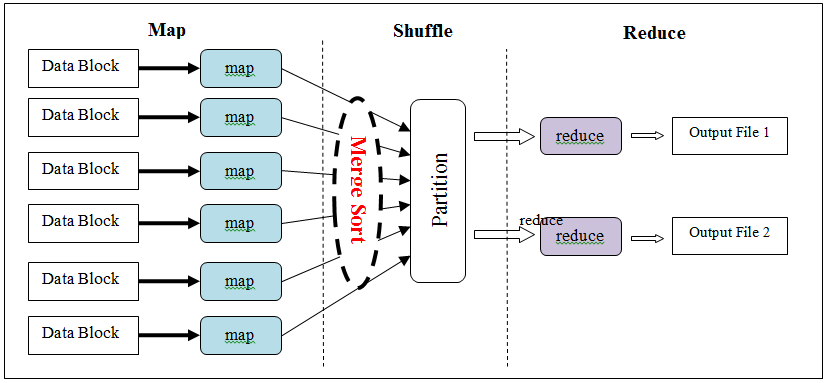
\includegraphics[width=\textwidth]{figs/5163os_01_02.png}
  \caption{Anatomy of a MapReduce job}\label{fig:mapred.job}
\end{figure} 

%%% \verb|Insert image 5163os_01_02.png|
\subsection*{There's more}
HDFS has two types of nodes, NameNode\index{NameNode} and DataNode. A NameNode keeps track of the filesystem metadata such as the locations of data blocks. For efficiency reasons, the metadata is kept in the main memory of a master machine. A DataNode holds physical data blocks, and communicates with clients for data reading and writing. In addition, it periodically reports a list of its hosting blocks to the NameNode in the cluster for verification and validation purposes.

The MapReduce framework has two types of nodes, master node and slave node. Jobtracker is the daemon on a master node, and Tasktracker is the daemon on a slave node. The master node is the manager node of MapReduce jobs. It splits a job into smaller tasks, which will be assigned by the JobTracker to TaskTrackers on slave nodes to run. When a slave node receives a task, its Tasktracker will fork a java process to run the task. Meanwhile, the Tasktracker is also responsible for tracking and reporting the progress of individual tasks.
\subsubsection*{Hadoop Common}
Hadoop common is a collection of components and interfaces for the foundation of Hadoop based Big Data platform. It provides the following components:
\begin{itemize}
  \item Distributed filesystem and I/O operation interfaces
  \item General parallel computation interfaces
  \item Logging
  \item Security management
\end{itemize}
\subsubsection*{Apache HBase}
Apache HBase\index{HBase} is an open source, distributed, versioned and column oriented data store. It was built on top of Hadoop and HDFS. HBase supports random, real time access to Big Data. It can scale to host very large table, containing billions of rows and millions of columns. More documentation about HBase can be obtained from \href{http://hbase.apache.org}{HBase @ Apache}.
\subsubsection*{Apache Mahout}
Apache Mahout\index{Mahout} is an open source scalable machine learning library based on Hadoop. It has a very active community and is still under development. Currently, the library supports four use cases: recommendation mining, clustering, classification and frequent item set mining. More documentation of Mahout can be obtained from \href{http://mahout.apache.org}{Mahout}.
\subsubsection*{Apache Pig}
Apache Pig\index{Pig} is a high level system for expressing Big Data analysis programs. It supports Big Data by compiling the Pig statements into a sequence of MapReduce jobs. Pig uses Pig Latin as the programming language, which is extensible and easy to use. More documentation about Pig can be found from \href{http://pig.apache.org}{Pig}.
\subsubsection*{Apache Hive}
Apache Hive\index{Hive} is a high level system for the management and analysis of Big Data stored in Hadoop based systems. It uses a SQL-like language called HiveQL. Similar to Apache Pig, the Hive runtime engine translates HiveQL statements into a sequence of MapReduce jobs for execution. More information about Hive can be obtained from \href{http://hive.apache.org}{Hive}.
\subsubsection*{Apache ZooKeeper}
Apache ZooKeeper\index{ZooKeeper} is a centralized coordination service for large scale distributed systems. It maintains the configuration and naming information and provides distributed synchronization and group services for applications in distributed systems. More documentation about ZooKeeper can be obtained from \href{http://zookeeper.apache.org}{ZooKeeper}.
\subsubsection*{Apache Oozie}
Apache Oozie\index{Oozie} is a scalable workflow management and coordination service for Hadoop jobs. It is data aware and coordinates jobs based on their dependencies. In addition, Oozie has been integrated with Hadoop and can support all types of Hadoop jobs. More information about Oozie can be obtained from \href{http://oozie.apache.org}{Oozie}.
\subsubsection*{Apache Sqoop}
Apache Sqoop\index{Sqoop} is a tool for moving data between Apache Hadoop and structured data stores such as relational databases. It provides command line suites to transfer data from relational database to HDFS and vice versa. More information about Apache Sqoop can be found at \href{http://sqoop.apache.org}{Sqoop}.
\subsubsection*{Apache Flume}
Apache Flume\index{Flume} is a tool for collecting log data in distributed systems. It has a flexible yet robust and fault tolerant architecture that streams data from log servers to Hadoop. More information can be obtained from \href{http://flume.apache.org}{Flume}.
\subsubsection*{Apache Avro}
Apache Avro\index{Avro} is a fast, feature rich data serialization system for Hadoop. The serialized data is coupled with the data schema, which facilitate its processing with different programming languages.  More information about Apache Avro can be found at \href{http://avro.apache.org}{Avro}.
\section{Choosing from Hadoop alternatives}
Although Hadoop has been very successful for most of the Big Data problems, it is not an optimal choice in many situations. In this recipe, we will introduce a few Hadoop alternatives.
\subsection*{Getting ready}
Hadoop has the following drawbacks as a Big Data platform:
\begin{itemize}
  \item As open source software, Hadoop is difficult to configure and manage, mainly due to the instability of the software and the lack of properly maintained documentation and technical support.
  \item Hadoop is not an optimal choice for real time, responsive Big Data applications.
  \item Hadoop is not a good fit for large graph data sets.
\end{itemize}

Because of the above drawbacks as well as other reasons such as special data processing requirements, we need to make an alternative choice.
\begin{info} 
Tip: \\
Hadoop is not a good choice for data that is not categorized as Big Data. For example, data that has the following properties: small data sets and data sets with processing that requires transaction and synchronization.
\end{info} 

\subsection*{How to do it}
We can choose Hadoop alternatives with the following guidelines:
\begin{enumerate}
  \item Choose Enterprise Hadoop if there is no qualified Hadoop administrator while there is sufficient budget for deploying a Big Data platform.
  \item Choose Spark or Storm if an application requires real time data processing.
  \item Choose GraphLab if an application requires handling of large graph data sets.
\end{enumerate}
\subsection*{How it works}
Enterprise Hadoop refers to Hadoop distributions by some Hadoop oriented companies. Compared with the community Hadoop releases, Enterprise Hadoop distributions are enterprise ready, easy to configure and sometimes new features are added. In addition, the training and support services provided by these companies make it much easier for organizations to adopt the Hadoop Big Data platform. Famous Hadoop oriented companies include: Cloudera, Horntonworks, MapR and Hadapt etc.
\begin{itemize}
  \item Cloudera is one of the most famous companies that are doing Enterprise Hadoop Big Data solutions. It provides Hadoop consulting, training and certification services. It is also one of the biggest contributors of the Hadoop code base. Their Big Data solution uses Cloudera Desktop as the cluster management interface. You can learn more from www.cloudera.com.
  \item Hortonworks and MapR both are providing featured Hadoop distributions and Hadoop based Big Data solutions. You can get more details from \url{www.hortonworks.com} and \url{www.mapr.com}.
  \item Hadapt differentiates itself from the other Hadoop oriented companies by the goal of integrating structured, semi-structured and unstructured data into a uniform data operation platform. Hadapt unifies SQL and Hadoop and makes it easy to handle different varieties of data. You can learn more at \href{http://hadapt.com/}{Hadapt}.
  \item Spark is a real time in-memory Big Data processing platform. It can be up to 40 times faster than Hadoop. So it is ideal for iterative and responsive Big Data applications. Besides, Spark can be integrated with Hadoop, and the Hadoop compatible storage APIs enables it to access any Hadoop supported systems. More information about Spark can be learned from \href{http://spark-project.org/}{Spark}.
  \item Storm is another famous real time Big Data processing platform. It is developed and open sourced by Twitter. For more information, please check \href{http://storm-project.net/}{Storm}.
  \item GraphLab is an open source distributed system developed at Carnegie Mellon University. It was targeted for handling sparse iterative graph algorithms. For more information, please visit: \href{http://graphlab.org/}{GraphLab home page}. The MapReduce framework parallels computation by splitting data onto a number of distributed nodes. Some large natural graph data such as social network data has the problem of being hard to partition and thus hard to split for Hadoop parallel processing. The performance can be severely panelized if Hadoop is used.
  \item Other Hadoop-like implementations include \href{http://mapreduce.stanford.edu/}{Phoenix}, which is a shared memory implementation of the MapReduce data processing framework and \href{http://code.google.com/p/haloop/}{HaLoop}, which is a modified version of Hadoop for iterative data processing.
\end{itemize}

\begin{warning}
Warning! \\
Phoenix and HaLoop do not have an active community and they are not recommended for production deployment.
\end{warning} 

\subsection*{There's more...}
As the Big Data problem floods the whole world, many systems have been designed to deal with the problem. Two famous such systems that do not follow the map-reduce route are Message Passing Interface (MPI) and High Performance Cluster Computing (HPCC).
\begin{description}
  \item{MPI\index{MPI}} is a library specification for message passing. Different from Hadoop, MPI was designed for high performance on both massively parallel machines and on workstation clusters. In addition, MPI lacks fault tolerance and performance will be bounded when data becomes large. More documentation about MPI can be found at \href{http://www.mpi-forum.org/}{MPI}.
  \item{HPCC\index{HPCC}} is an open source Big Data platform developed by HPCC systems, which was acquired by LexisNexis Risk Solutions. It achieves high performance by clustering commodity hardware. The system includes configurations for both parallel batch processing and high performance online query applications using indexed data files. The HPCC platform contains two cluster processing subsystems: Data Refinery subsystem and Data Delivery subsystem. The Data Refinery subsystem is responsible for the general processing of massive raw data and the Data Delivery subsystem is responsible for the delivery of clean data for online queries and analytics. More information about HPCC can be found at \href{http://hpccsystems.com/}{HPCC}.
\end{description}
